\documentclass[11pt, oneside]{article}   	% use "amsart" instead of "article" for AMSLaTeX format
\usepackage{geometry}                		% See geometry.pdf to learn the layout options. There are lots.
\geometry{letterpaper}                   		% ... or a4paper or a5paper or ... 
%\geometry{landscape}                		% Activate for for rotated page geometry
%\usepackage[parfill]{parskip}    		% Activate to begin paragraphs with an empty line rather than an indent
\usepackage{graphicx}				% Use pdf, png, jpg, or eps§ with pdflatex; use eps in DVI mode
								% TeX will automatically convert eps --> pdf in pdflatex		
\usepackage{amssymb}

\title{Brief Article}
\author{The Author}
%\date{}							% Activate to display a given date or no date

\begin{document}
\maketitle
%\section{}
%\subsection{}

\section{True Solution of Transport Equation}


As a solution for the transport equation of form

\begin{equation}
\frac{\delta u}{\delta t} = \frac{\delta u}{\delta x} + \frac{\delta u}{\delta y}
\end{equation}
with a given initial conditions, $u_0(x,y)$, and homogenous dirichet boundary conditions we propose a solution of the following form:
\begin{equation}
u(x,y,t) = u_0(x-vt,y-vt)
\label{proposal}
\end{equation}
Calculating the partial derivatives found in the transport equation we get
\begin{equation}
\frac{\delta u}{\delta t} =(-v) \frac{\delta u_0(x,y)}{\delta x} +(-v) \frac{\delta u_0(x,y)}{\delta y} 
\end{equation}

\begin{equation}
\frac{\delta u}{\delta x} = \frac{\delta u_0(x,y)}{\delta x} ,\frac{\delta u}{\delta y} = \frac{\delta u_0(x,y)}{\delta y} 
\end{equation}
Filling this then in the transport equation gives

\begin{equation}
-v\frac{\delta u_0}{\delta x}-v\frac{\delta u_0}{\delta y} = \frac{\delta u_0}{\delta x}+\frac{\delta u_0}{\delta y} 
\end{equation}

which fits when $v=-1$ and so our solution is
\begin{equation}
u(x,y,t)=u_0(x+t,y+t)
\end{equation}

\section{error analysis of the transport problem}

The truncation error for the upwind scheme with $a=1$ can be found to be

\begin{equation}
T_j^n = -\frac{1}{2}(1-\nu)\Delta x u_{xx} + ...
\end{equation}
Which is forst order in $\Delta x$, and therefor, under constant $\nu$, also first order in $\Delta t$.

We then now that the maximum error $E^n$ at a point in time $n$ is bound by a function of the same order. And this is what we see in figure \ref{errororrrTransport}

\begin{figure}[htbp] %  figure placement: here, top, bottom, or page
   \centering
   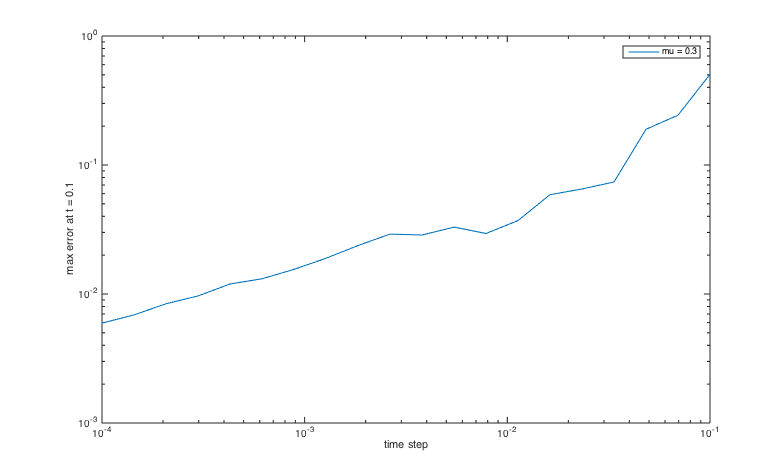
\includegraphics[width=15cm]{errororrrTransport} 
   \caption{The maximum error at time = 0.1 in function of the tilmestep at a constant $\nu$ of 0.3 }
   \label{errororrrTransport}
\end{figure}


\end{document}  

